\section{通讯与同步}
在第 4 章中,我们讨论了使用基本数据并行Kernel或显式 ND 范围Kernel来表达并行性的方法。 
我们讨论了基本数据并行Kernel如何独立地将相同的操作应用于每条数据。 
我们还讨论了显式 ND 范围Kernel如何将执行范围划分为Work-Items的Work-Groups。

在本章中,我们将重新审视如何在不断追求并行思考的过程中将问题分解为小块的问题。 
本章提供了有关显式 ND 范围Kernel的更多详细信息,并描述了如何使用Work-Items分组来提高某些类型算法的性能。 
我们将描述Work-Items组如何为并行工作的执行方式提供额外的保证,并且我们将介绍支持Work-Items分组的语言功能。 
在第 15、16 和 17 章中优化特定设备的程序以及在第 14 章中描述常见并行模式时,许多想法和概念非常重要。

\subsection{Work-Groups和Work-Items}
回想一下第 4 章,显式 ND 范围Kernel将Work-Items组织到Work-Groups中,
并且同一Work-Groups中的所有Work-Items都有额外的调度保证。 
这个属性很重要,因为它意味着Work-Groups中的Work-Items可以合作解决问题。

\begin{figure}[H]
	\centering
	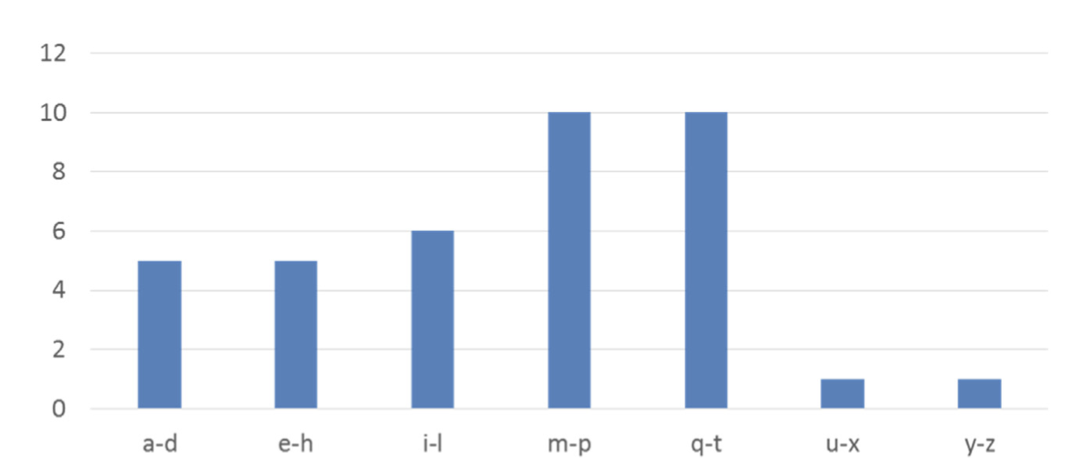
\includegraphics[width=0.9\textwidth]{figs/F9.1.png}
	\caption{\textit{大小 (8, 8) 的二维 ND 范围分为四个大小为 (4,4) 的Work-Groups }}
\end{figure}

图 9-1 显示了划分为Work-Groups的 ND 范围,其中每个Work-Groups由不同的颜色表示。 
每个Work-Groups中的Work-Items可以安全地与共享相同颜色的其他Work-Items进行通信。

无法保证不同Work-Groups中的Work-Items会同时执行,
因此具有一种颜色的Work-Items无法与具有不同颜色的Work-Items可靠地通信。 
如果一个Work-Items尝试与当前未执行的另一Work-Items通信,则Kernel可能会死锁。 
由于我们希望Kernel能够完成执行,因此我们必须确保当一个Work-Items与另一Work-Items通信时,
它们位于同一个Work-Groups中。

\subsection{高效通讯的基石}
本节描述支持组中Work-Items之间高效通信的构建块。 
有些是基本构建块,可以构建自定义算法,而另一些则是更高级别的,描述许多Kernel使用的常见操作。

\subsubsection{通过屏障(Barriers)进行同步}
通信最基本的组成部分是Barrier功能。 Barrier功能有两个主要目的:

首先,Barrier功能同步组中Work-Items的执行。 
通过同步执行,一个Work-Items可以确保同一组中的另一个Work-Items在使用该操作的结果之前已完成该操作。 
或者,在另一个Work-Items使用操作结果之前,给一个Work-Items时间来完成其操作。

其次,Barrier函数同步每个Work-Items如何查看内存状态。 
这种类型的同步操作称为强制内存一致性或隔离内存(更多详细信息请参阅第 19 章)。 
内存一致性至少与同步执行一样重要,
因为它确保在Barrier之前执行的内存操作的结果对于Barrier之后的其他Work-Items是可见的。 
如果没有内存一致性,一个Work-Items中的操作就像森林中的一棵树倒下一样,其他Work-Items可能会也可能听不到声音!

\begin{figure}[H]
	\centering
	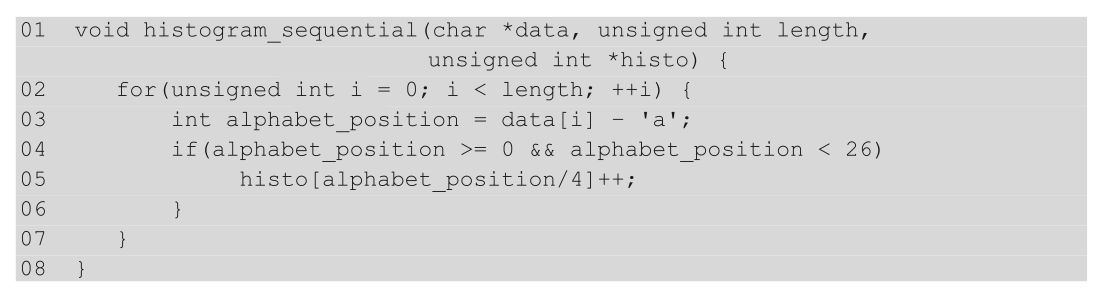
\includegraphics[width=0.9\textwidth]{figs/F9.2.png}
	\caption{\textit{组中的四个Work-Items在 Barrier 函数处同步 }}
\end{figure}

图 9-2 显示了一组中在Barrier函数处同步的四个Work-Items。 
尽管每个Work-Items的执行时间可能不同,但在所有Work-Items都执行Barrier之前,
没有任何Work-Items可以执行越过Barrier。 
执行Barrier函数后,所有Work-Items都具有一致的内存视图。

\begin{remark}[为什么默认情况下内存不一致?]
对于许多程序员来说,内存一致性的概念(以及不同的Work-Items可以具有不同的内存视图)可能会让人感到非常奇怪。
如果默认情况下所有Work-Items的所有内存都是一致的,那不是更容易吗?简短的回答是它会,但实施起来也会非常昂贵。
通过允许Work-Items具有不一致的内存视图,并且只要求在程序执行期间定义的点具有内存一致性,
加速器硬件可能更便宜,性能更好,或两者兼而有之。
\end{remark}

因为Barrier函数同步执行,所以组中的所有Work-Items都执行Barrier或者组中没有Work-Items执行Barrier是至关重要的。 
如果组中的某些Work-Items围绕任何 Barrier函数分支,
则组中的其他Work-Items可能会永远在 Barrier处等待,或者至少直到用户放弃并终止程序!

\begin{remark}[集体函数]
当某个函数需要由组中的所有Work-Items执行时,它可以称为集体函数,因为该操作是由组执行的,
而不是由组中的单个Work-Items执行的。
Barrier 函数并不是 SYCL 中唯一可用的集体函数。本章稍后将介绍其他集体函数。
\end{remark}

\subsubsection{Work-Groups本地内存}
Work-Groups Barrier功能足以协调Work-Groups中Work-Items之间的通信,但通信本身必须通过内存进行。 
通信可以通过 USM 或Buffer进行,但这可能不方便且效率低下:它需要专门的通信分配,并且需要在Work-Groups之间划分分配。

为了简化Kernel开发并加速Work-Groups中Work-Items之间的通信,SYCL定义了一个特殊的本地内存空间,
专门用于Work-Groups中Work-Items之间的通信。

\begin{figure}[H]
	\centering
	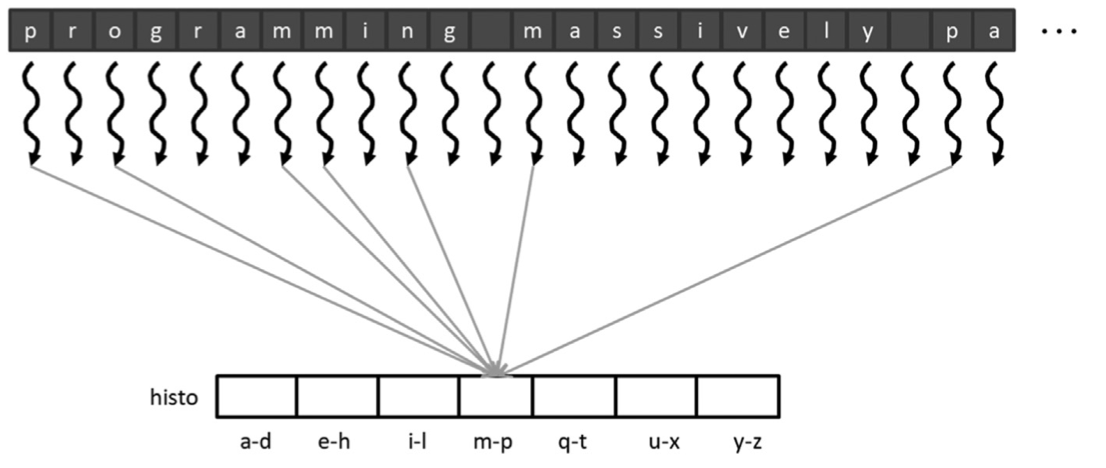
\includegraphics[width=0.9\textwidth]{figs/F9.3.png}
	\caption{\textit{每个Work-Groups可以访问所有全局内存,但只能访问自己的本地内存 }}
\end{figure}

图 9-3 显示了两个Work-Groups。 两个Work-Groups都可以访问USM和全局内存空间中的Buffer。 
每个Work-Groups可以访问自己的本地内存空间中的变量,但不能访问另一个Work-Groups本地内存中的变量。

当Work-Groups开始时,其本地内存的内容未初始化,并且在Work-Groups执行完成后本地内存不会保留。 
由于这些属性,本地内存只能在Work-Groups执行时用于临时存储。

对于某些设备,例如对于许多CPU设备,本地存储器是软件抽象并且使用与全局存储器相同的存储器子系统来实现。 
在这些设备上,使用本地内存主要是一种方便的通信机制。 
某些编译器可能会使用内存空间信息进行编译器优化,但在其他情况下,
使用本地内存进行通信从根本上来说不会比通过这些设备上的全局内存进行通信更好。

对于其他设备,例如许多 GPU 设备,有专用的本地内存资源。 
在这些设备上,通过本地内存进行通信比通过全局内存进行通信性能更好。

\begin{remark}
	使用本地内存时,Work-Groups中Work-Items之间的通信可以更方便、更快捷!
\end{remark}

我们可以使用设备查询 info::device::local\_mem\_type 来确定加速器是否具有用于本地内存的专用资源,
或者本地内存是否被实现为全局内存的软件抽象。 
有关查询设备属性的更多信息,请参阅第 12 章;有关 CPU、GPU 和 FPGA 的本地内存通常如何实现的更多信息,
请参阅第 15、16 和 17 章。

\subsection{使用Work-Groups Barrier和本地内存}
现在我们已经确定了Work-Items之间有效通信的基本构建块,我们可以描述如何在Kernel中表达Work-Groups Barrier和本地内存。 
请记住,Work-Items之间的通信需要Work-Items分组的概念,因此这些概念只能针对 ND 范围Kernel来表达,
并且不包含在基本数据并行Kernel的执行模型中。

本章将通过介绍执行矩阵乘法的Work-Groups中的Work-Items之间的通信,
建立在第 4 章中介绍的朴素矩阵乘法Kernel示例的基础上。 
在许多设备上(但不一定是所有设备!)通过本地内存进行通信将提高矩阵乘法Kernel的性能。

\begin{remark}[关于矩阵乘法的说明]
在本书中,矩阵乘法Kernel用于演示Kernel的变化如何影响性能。尽管使用本章中描述的技术可以在许多设备上提高矩阵乘法性能,
但矩阵乘法是一项非常重要且常见的操作,因此许多供应商已经实现了矩阵乘法的高度调整版本。
供应商投入大量时间和精力为特定设备实现和验证功能,在某些情况下,
可能会使用在标准并行Kernel中难以或不可能使用的功能或技术。
\end{remark}

\begin{remark}[使用供应商提供的库!]
当供应商提供函数的库实现时,使用它几乎总是有益的,而不是将函数重新实现为并行Kernel!
对于矩阵乘法,可以将oneMKL视为英特尔工具包的一部分,以提供适合SYCL程序员的C++解决方案。
\end{remark}

\begin{figure}[H]
	\centering
	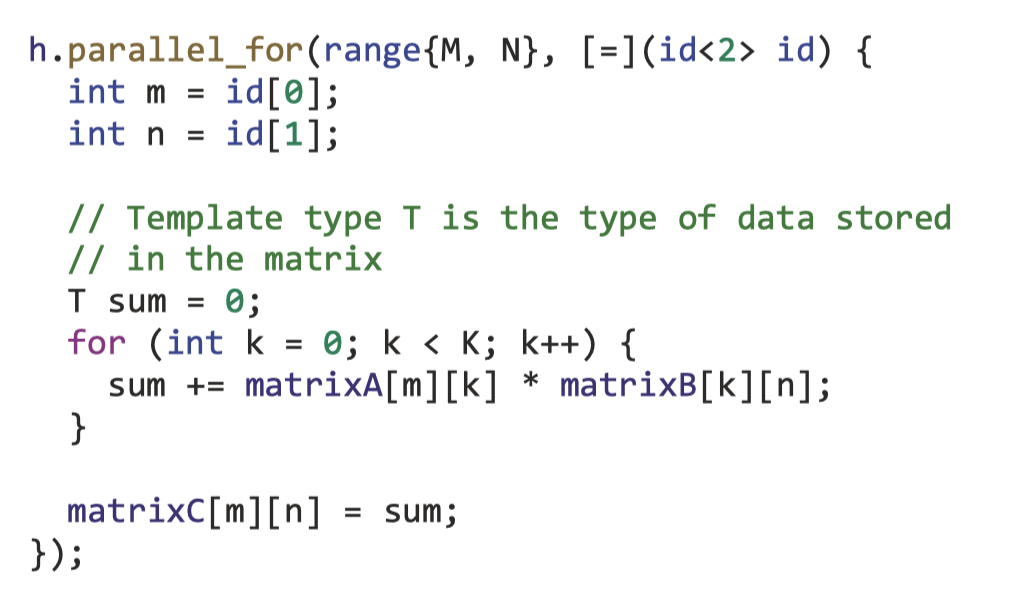
\includegraphics[width=0.9\textwidth]{figs/F9.4.png}
	\caption{\textit{第 4 章中的朴素矩阵乘法Kernel }}
\end{figure}

图 9-4 显示了我们将从中开始的朴素矩阵乘法Kernel,类似于第 4 章中的矩阵乘法Kernel。
对于该Kernel以及本章中的所有矩阵乘法Kernel,T 是一个模板类型,指示类型 存储在矩阵中的数据的数量,
例如 32 位浮点型或 64 位双精度型。

在第4章中,我们观察到矩阵乘法算法具有高度的重用性,并且对Work-Items进行分组可以提高访问的局部性,
因此也可以提高缓存命中率。 
在本章中,我们修改后的矩阵乘法Kernel将不再依赖隐式缓存行为来提高性能,而是使用本地内存作为显式缓存,以保证访问的局部性。

\begin{remark}
	对于许多算法,将本地内存视为显式缓存会很有帮助。
\end{remark}

\begin{figure}[H]
	\centering
	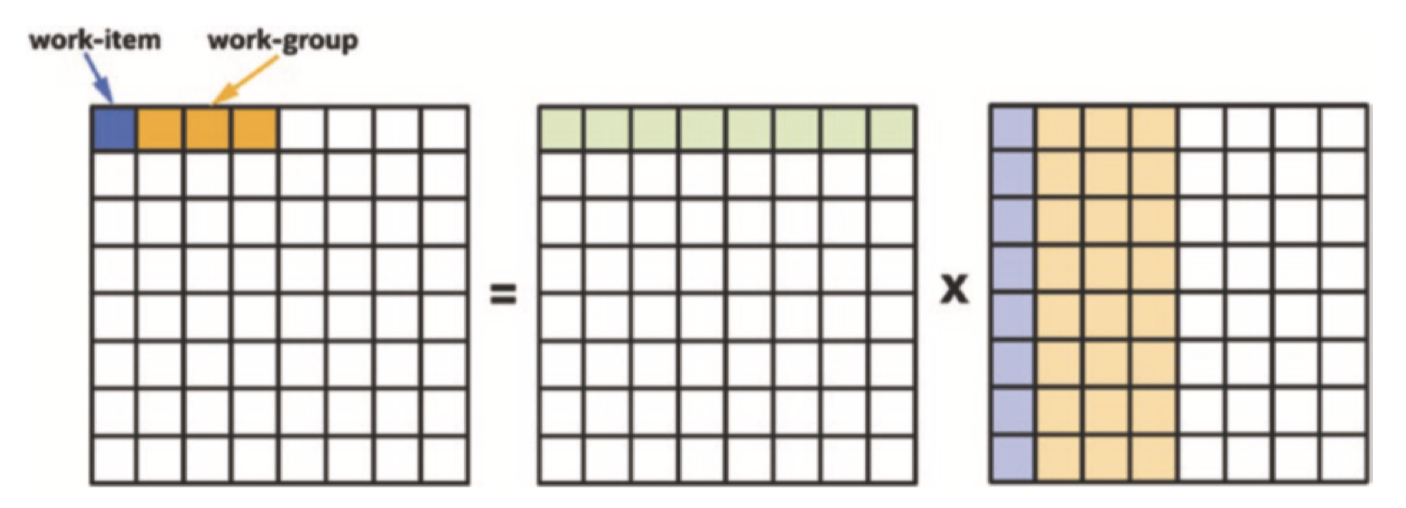
\includegraphics[width=0.9\textwidth]{figs/F9.5.png}
	\caption{\textit{矩阵乘法到Work-Groups和Work-Items的映射 }}
\end{figure}

图 9-5 是第 4 章的修改图,显示了由单行组成的Work-Groups,这使得使用本地内存的算法更容易理解。 
观察到,对于结果矩阵的一行中的元素,每个结果元素都是使用来自输入矩阵之一的唯一数据列计算的(以蓝色和橙色显示)。 
由于该输入矩阵没有数据共享,因此它不是本地内存的理想候选者。 
但请注意,该行中的每个结果元素都访问另一个输入矩阵中完全相同的数据(以绿色显示)。 
由于这些数据被重用,因此它是从Work-Groups本地内存中受益的绝佳候选者。

因为我们想要乘以可能非常大的矩阵,并且Work-Groups本地内存可能是有限的资源,
所以我们修改后的Kernel将处理每个矩阵的子部分,我们将其称为矩阵图块。 
对于每个图块,我们修改后的Kernel会将图块的数据加载到本地内存中,
同步组中的Work-Items,然后从本地内存而不是全局内存加载数据。 
第一个图块访问的数据如图 9-6 所示。

\begin{figure}[H]
	\centering
	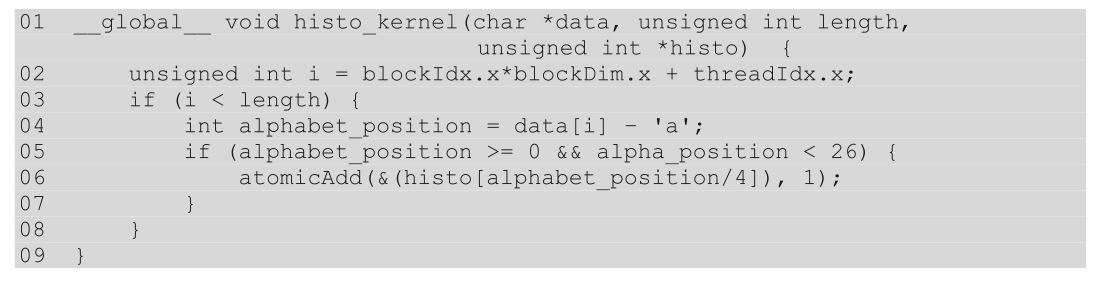
\includegraphics[width=0.9\textwidth]{figs/F9.6.png}
	\caption{\textit{处理第一个图块:绿色输入数据(X的左边)被重用并从本地内存中读取,
蓝色和橙色的输入数据(X的右边)从全局内存中读取 }}
\end{figure}

在我们的Kernel中,我们选择了与Work-Groups大小相等的图块大小。 
这不是必需的,但因为它简化了本地内存的传入或传出,所以选择Work-Groups大小的倍数的图块大小是常见且方便的。

\subsubsection{ND 范围Kernel中的Work-Groups Barrier和本地内存}
本节介绍如何在 ND 范围Kernel中表达Work-Groups Barrier和本地内存。 
对于 ND 范围Kernel,表示是显式的:Kernel声明本地访问器并对其进行操作,
该本地访问器表示本地地址空间中的分配,并调用Barrier函数来同步Work-Groups中的Work-Items。

\paragraph{本地访问器}

要声明本地内存用于 ND 范围Kernel,请使用本地访问器。 
与其他访问器对象一样,本地访问器是在命令组处理程序中构造的,但与第 3 章和第 7 章中讨论的访问器对象不同,
本地访问器不是从Buffer对象创建的。 相反,本地访问器是通过指定类型和描述该类型元素数量的范围来创建的。 
与其他访问器一样,本地访问器可以是一维、二维或三维的。 图 9-7 演示了如何声明本地访问器并在Kernel中使用它们。

\begin{figure}[H]
	\centering
	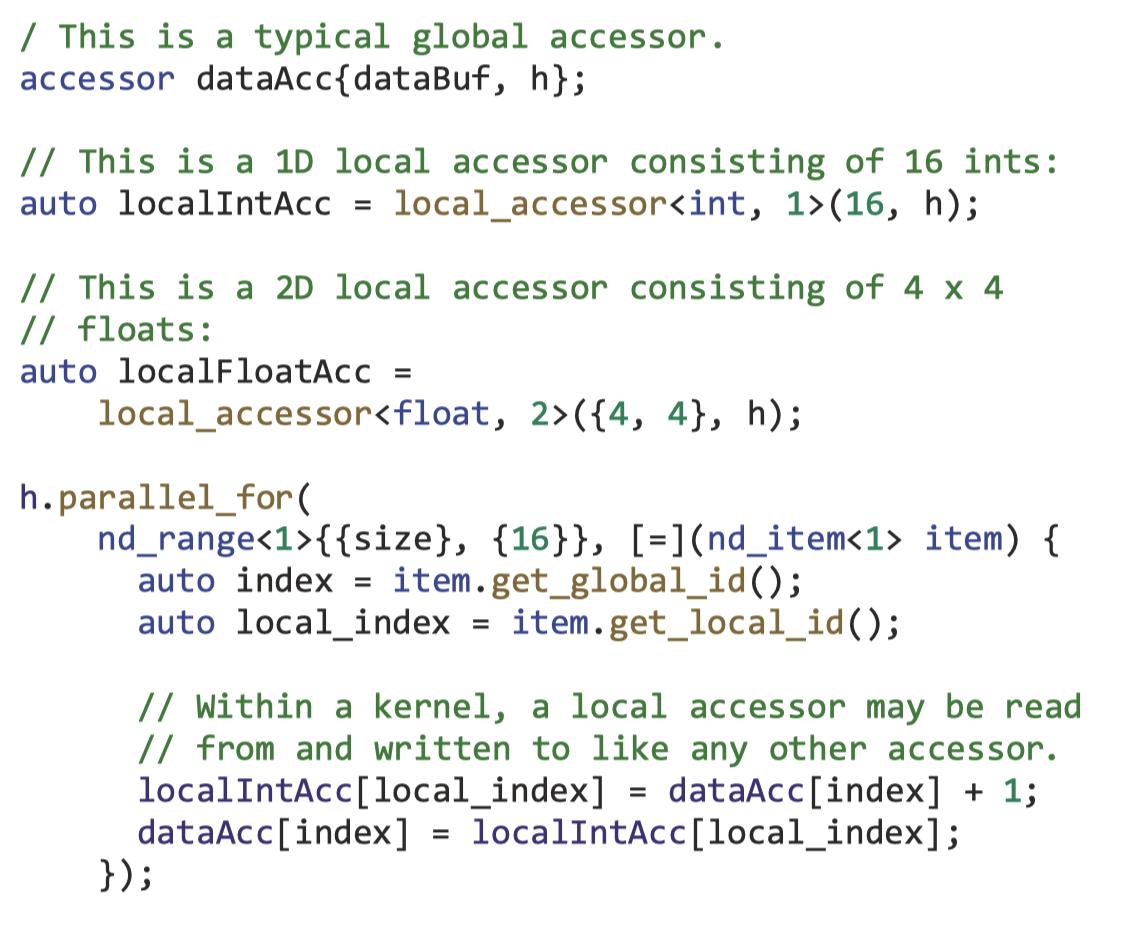
\includegraphics[width=0.9\textwidth]{figs/F9.7.png}
	\caption{\textit{声明和使用本地访问器取 }}
\end{figure}

请记住,本地内存在每个Work-Groups开始时未初始化,并且在每个Work-Groups完成后不会保留。 
这意味着本地访问器必须始终是 read\_write,否则Kernel将无法分配本地内存的内容或查看分配的结果。 
不过,本地访问器可以选择是原子的,在这种情况下,通过访问器对本地存储器的访问是原子地执行的。 
第 19 章更详细地讨论了原子访问。

\paragraph{同步功能}

要同步 ND 范围KernelWork-Groups中的Work-Items,请使用代表Work-Groups的组调用 group\_barrier 函数。 
由于代表Work-Groups的组只能从 nd\_item 查询,而不能从 item 查询,
因此Work-Groups Barrier仅适用于 ND 范围Kernel,不适用于基本数据并行Kernel。

group\_barrier 函数接受一个附加的可选参数来描述Barrier执行的任何内存一致性操作的范围。 
当没有附加参数传递给 group\_barrier 函数时,Barrier函数将根据传入的组确定默认范围。 
默认范围通常是正确的,因此很少需要显式范围,但如果某些算法需要,可以扩大内存范围。

请注意,显式作用域仅影响由Barrier执行的内存操作,
并且在Barrier处同步执行的Work-Items集完全由传递给Barrier的组对象确定。 
我们无法通过将不同的内存范围传递给Barrier来同步更多或更少的Work-Items,
但我们可以通过将不同的组对象传递给Barrier来同步一组不同的Work-Items。

\paragraph{完整的 ND 范围Kernel示例}

现在我们知道如何声明本地内存访问器并使用Barrier函数同步对其的访问,
我们可以实现矩阵乘法的 ND 范围Kernel版本,它协调Work-Groups中Work-Items之间的通信,以减少全局流量 内存。 
完整的示例如图 9-8 所示。

\begin{figure}[H]
	\centering
	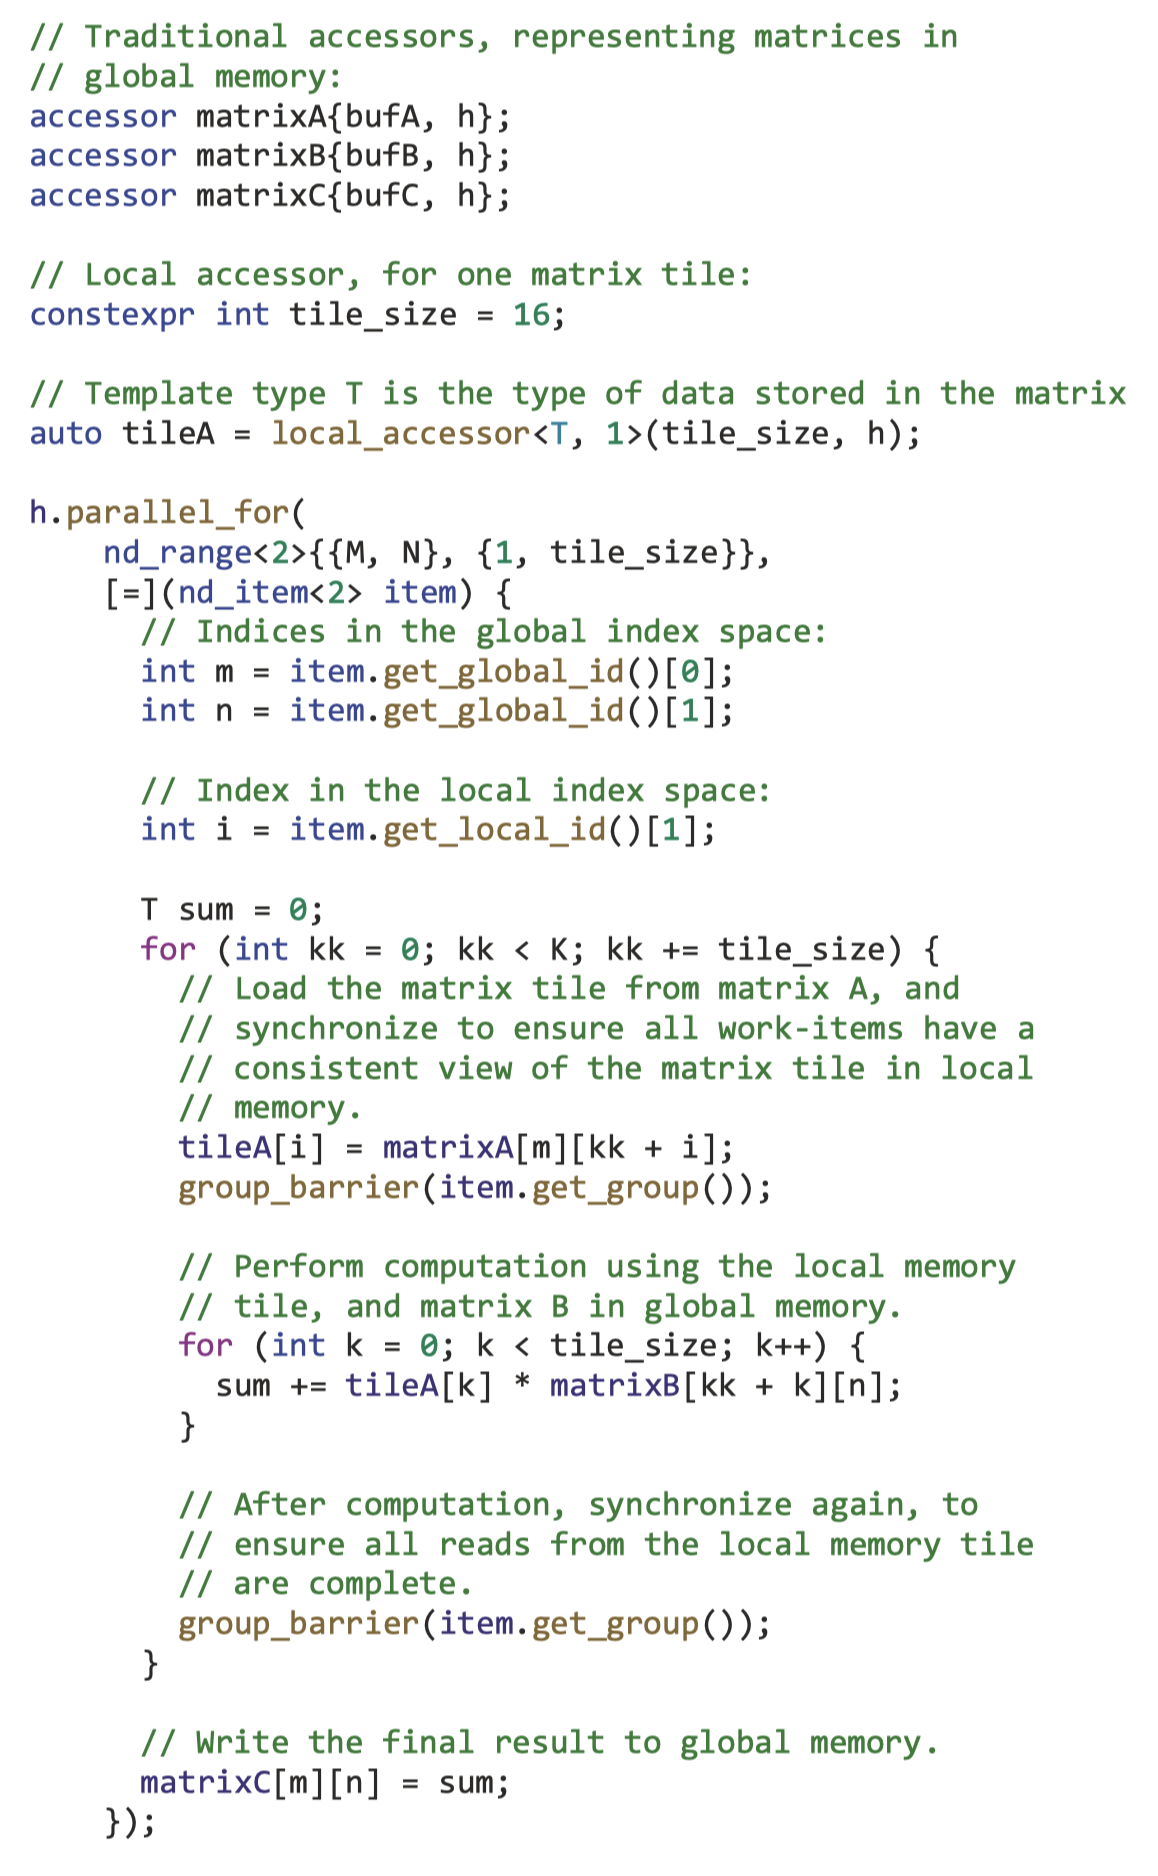
\includegraphics[width=0.9\textwidth]{figs/F9.8.png}
	\caption{\textit{用 ND 范围parallel\_for和Work-Groups本地存储器表达平铺矩阵乘法Kernel }}
\end{figure}

该Kernel中的主循环可以被认为是两个不同的阶段:
在第一阶段,Work-Groups中的Work-Items协作将共享数据从A矩阵加载到Work-Groups本地内存中; 
在第二个中,Work-Items使用共享数据执行自己的计算。 
为了确保所有Work-Items在进入第二阶段之前都已完成第一阶段,这两个阶段通过调用 group\_barrier 来分隔,
以同步Work-Groups中的所有Work-Items并提供内存栅栏。 
这种模式是一种常见的模式,在Kernel中使用Work-Groups本地内存几乎总是需要使用Work-Groups Barrier。

请注意,还必须调用 group\_barrier 来同步当前图块的计算阶段和下一个矩阵图块的加载阶段之间的执行。 
如果没有这种同步操作,当前矩阵图块的一部分可能会在另一Work-Items完成计算之前被Work-Groups中的一个Work-Items覆盖。 
一般来说,每当一个Work-Items在本地存储器中读取或写入由另一Work-Items读取或写入的数据时,就需要同步。 
在图 9-8 中,同步是在循环结束时完成的,但在每个循环迭代开始时进行同步也同样正确。

\subsection{Sub-Groups}
到目前为止,在本章中,Work-Items已通过Work-Groups本地内存交换数据并使用Work-Groups上
的 group\_barrier 函数进行同步,从而与Work-Groups中的其他Work-Items进行通信。

在第 4 章中,我们讨论了另一组Work-Items。 Sub-Groups是Work-Groups中由实现定义的Work-Items子集,
它们在相同的硬件资源上一起执行或具有额外的调度保证。 
因为实现决定如何将Work-Items分组为Sub-Groups,
所以Sub-Groups中的Work-Items可能能够比任意Work-Groups中的Work-Items更有效地通信或同步。

本节描述Sub-Groups中Work-Items之间通信的构建块。 
Sub-Groups还需要Work-Items分组的概念,因此Sub-Groups也需要 ND 范围Kernel,
并且不包含在基本数据并行Kernel的执行模型中。

\subsubsection{通过Sub-Groups Barrier进行同步}

\begin{figure}[H]
	\centering
	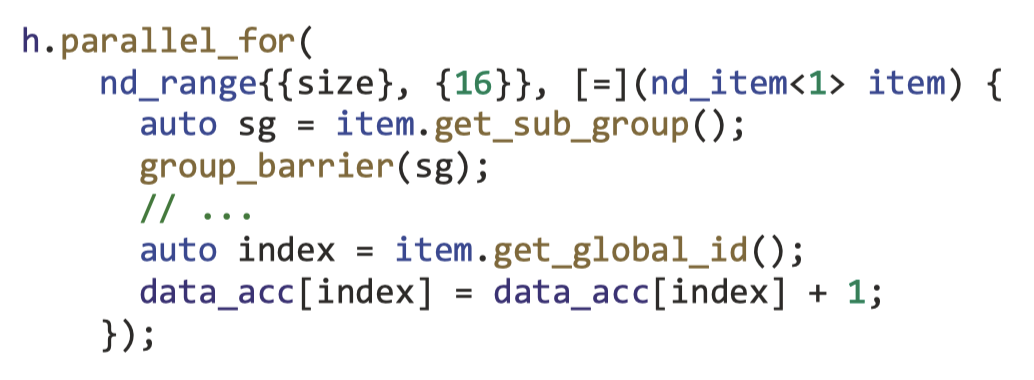
\includegraphics[width=0.9\textwidth]{figs/F9.9.png}
	\caption{\textit{查询和使用 sub\_group 类 }}
\end{figure}

正如Work-Groups中的Work-Items可以如何使用Work-Groups Barrier来同步一样,
Sub-Groups中的Work-Items可以使用Sub-Groups Barrier来同步。 
要执行Sub-Groups Barrier,请调用相同的 group\_barrier 函数,
但传递代表Sub-Groups而不是Work-Groups的组对象,如图 9-9 所示。 
与Work-Groups对象一样,可以从 ND 范围Kernel的 nd\_item 类查询表示Sub-Groups的组对象,但不能从基本数据并行项查询。

与Work-Groups Barrier一样,
Sub-Groups Barrier可以接受可选参数来扩大与Sub-Groups Barrier相关的任何内存操作的范围,
但这并不常见,在大多数情况下我们可以简单地使用默认内存范围。

\subsubsection{在Sub-Groups内交换数据}
与Work-Groups不同,Sub-Groups没有用于交换数据的专用存储空间。 
相反,Sub-Groups中的Work-Items可以通过Work-Groups本地存储器、
通过全局存储器或更常见地通过使用Sub-Groups集体功能来交换数据。

如前所述,集体函数是描述由一组Work-Items而不是单个Work-Items执行的操作的函数。 
由于Barrier同步功能是由一组Work-Items执行的操作,因此它是集体功能的一个示例。

其他集体功能表达了共同的沟通模式。 
我们将在本章后面详细描述许多集体函数的语义,但现在我们重点关注 group\_broadcast 集体函数,
我们将使用它来实现使用Sub-Groups的矩阵乘法。

\begin{figure}[H]
	\centering
	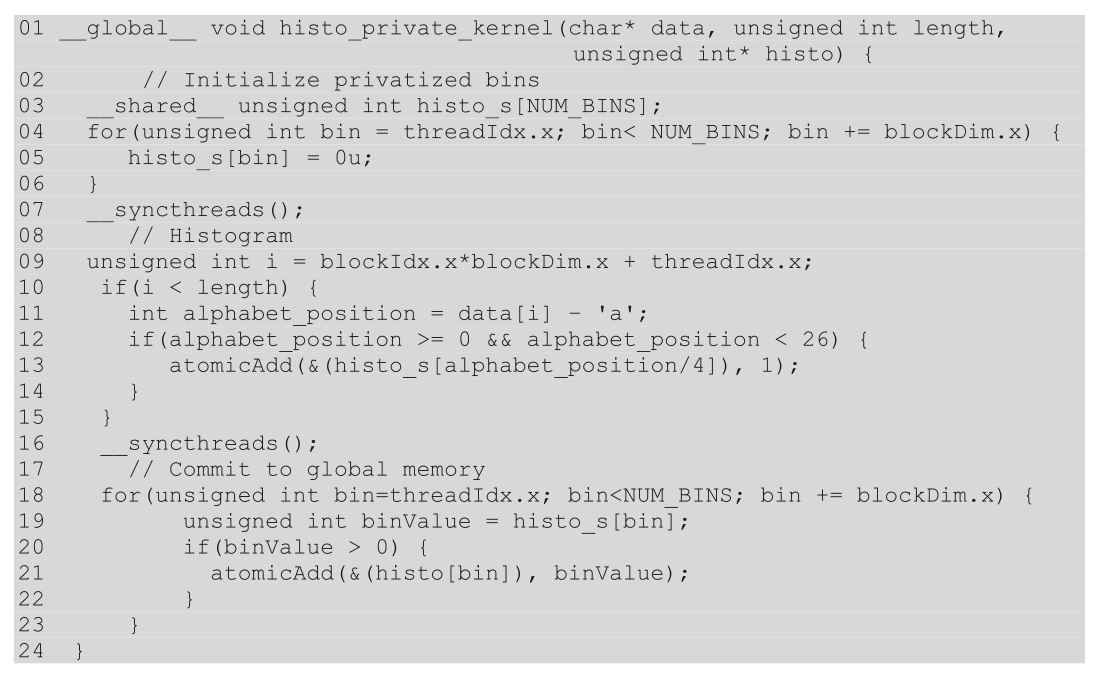
\includegraphics[width=0.9\textwidth]{figs/F9.10.png}
	\caption{\textit{广播函数 }}
\end{figure}

group\_broadcast 集体函数从组中的一个Work-Items获取一个值,并将其传递给组中的所有其他Work-Items。 
图 9-10 显示了一个示例。 
请注意,广播函数的语义要求标识组中要通信的值的 local\_id 对于组中的所有Work-Items必须相同,
以确保广播函数的结果对于所有Work-Items也相同 在组中。

\begin{figure}[H]
	\centering
	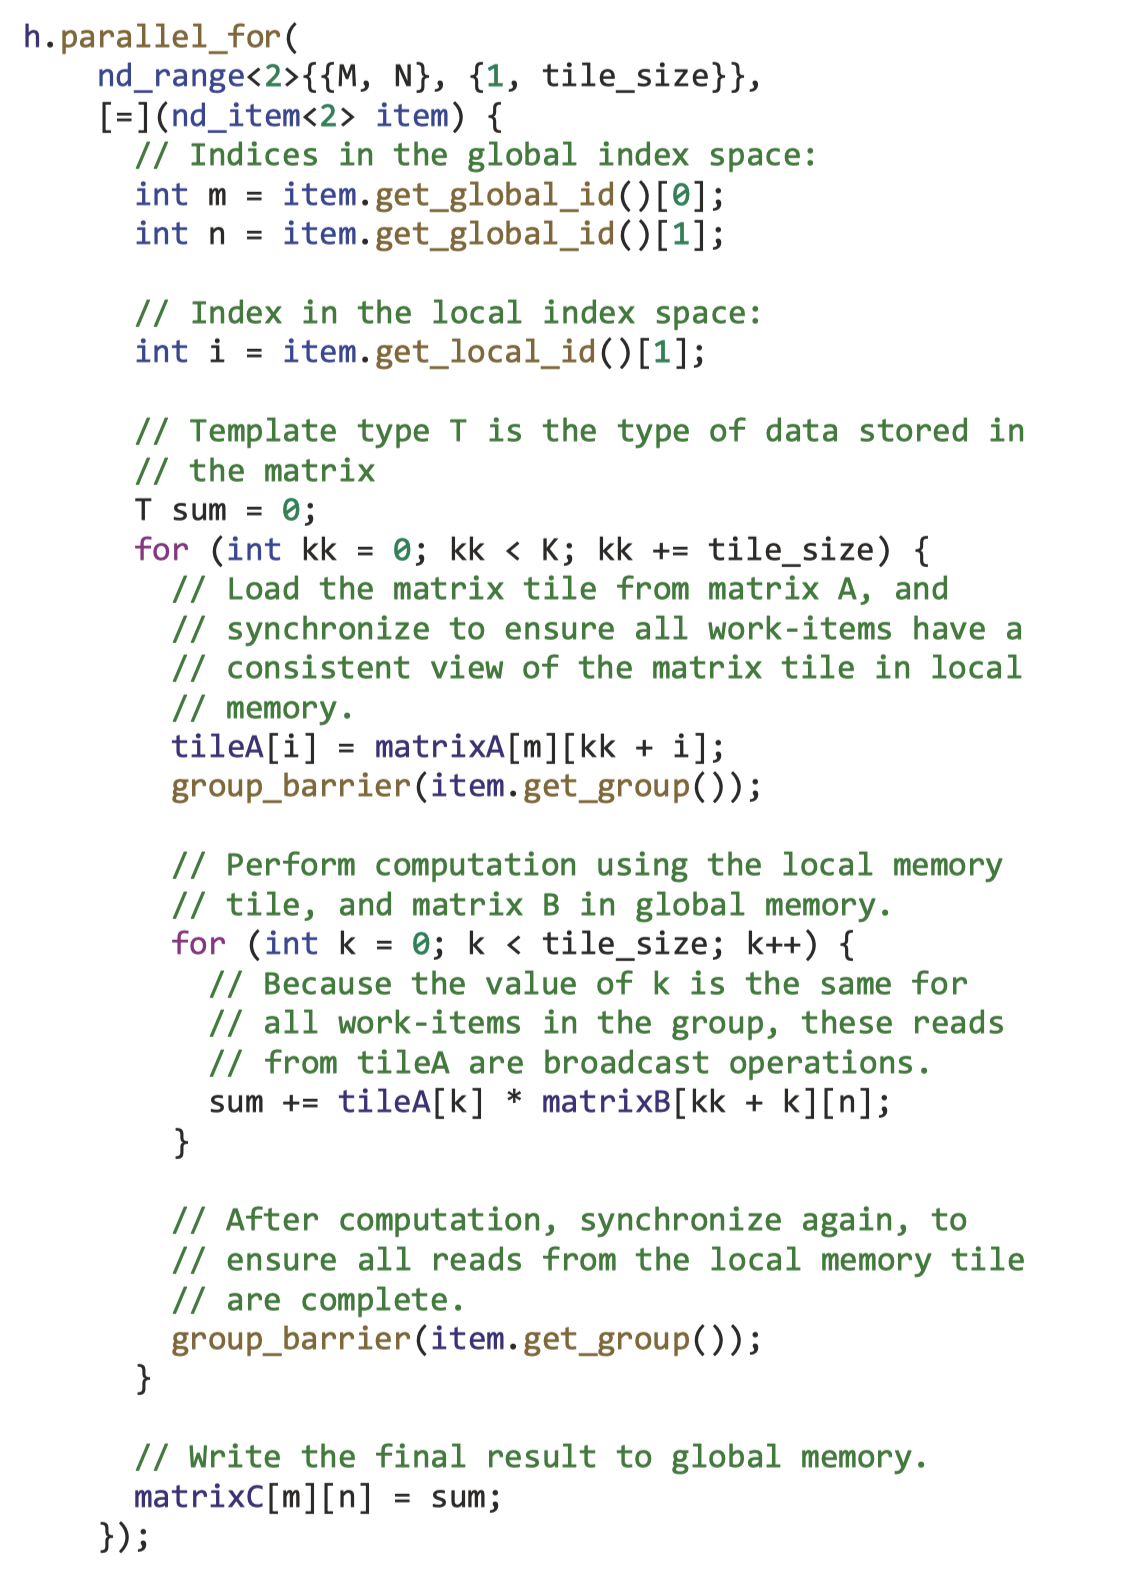
\includegraphics[width=0.9\textwidth]{figs/F9.11.png}
	\caption{\textit{矩阵乘法Kernel包括广播操作 }}
\end{figure}

如果我们查看本地内存矩阵乘法Kernel的最内层循环(如图 9-11 所示),
我们可以看到对矩阵图块的访问是广播操作,因为组中的每个Work-Items都读取相同的值 矩阵瓦片的。

我们将使用带有Sub-Groups对象的 group\_broadcast 函数来实现不需要Work-Groups本地内存或Barrier的矩阵乘法Kernel。 
在许多设备上,使用Work-Groups本地内存和Barrier,Sub-Groups广播比Work-Groups广播更快。

\subsubsection{完整Sub-Groups ND 范围Kernel示例}
\begin{figure}[H]
	\centering
	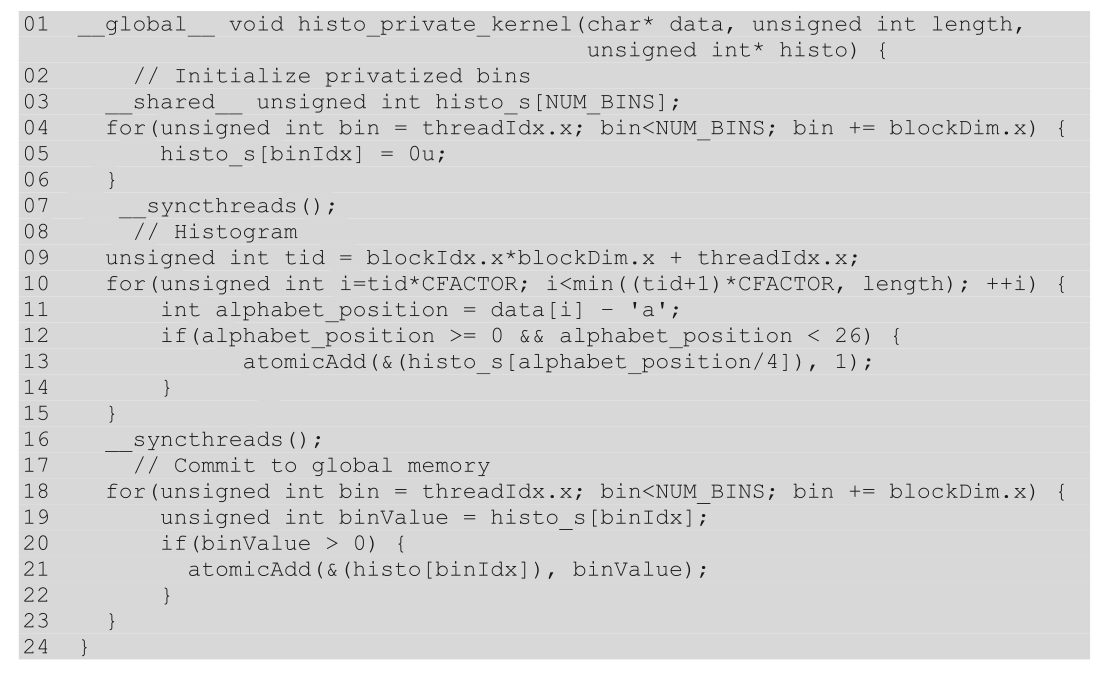
\includegraphics[width=0.9\textwidth]{figs/F9.12.png}
	\caption{\textit{用ND范围parallel\_for和Sub-Groups集体函数表示的平铺矩阵乘法核 }}
\end{figure}

图 9-12 是使用Sub-Groups实现矩阵乘法的完整示例。 
请注意,该Kernel不需要Work-Groups本地内存或显式同步,
而是使用Sub-Groups广播集体功能来在Sub-Groups中的Work-Items之间传达矩阵图块的内容。

\subsection{组函数和组算法}
在本章的“Sub-Groups”部分中,我们描述了集体功能以及集体功能如何表达常见的沟通模式。 
我们特别讨论了广播集体功能,它用于将值从组中的一个Work-Items传递到组中的其他Work-Items。 本节描述附加的集体功能。

尽管本节中描述的集体功能可以使用原子、Work-Groups本地内存和Barrier等功能直接在我们的程序中实现,
但许多设备都包含专用硬件来加速集体功能。 
即使设备不包含专用硬件,供应商提供的集体函数的实现也可能会针对其运行的设备进行调整,
因此调用内置集体函数通常会比我们编写的通用实现执行得更好 。

\begin{remark}
	将集体函数用于常见的通信模式,以简化代码并提高性能!
\end{remark}

\subsubsection{广播 Broadcast}
group\_broadcast 函数使组中的一个Work-Items能够与组中的所有其他Work-Items共享变量的值。 
广播功能的工作原理如图 9-10 所示。 Work-Groups和Sub-Groups都支持 group\_broadcast 功能。

\subsubsection{投票 Votes}
any\_of\_group、all\_of\_group 和 none\_of\_group 函数(以下称为“投票”函数)
使Work-Items能够比较其组中布尔条件的结果:如果条件对于其中至少一个Work-Items为真,则any\_of\_group 返回 true。 
如果组中所有Work-Items的条件都为 true,则 all\_of\_group 返回 true;
如果组中的所有Work-Items的条件为 false,则 none\_of\_group 返回 true。 
图 9-13 显示了示例输入的这两个函数的比较。

\begin{figure}[H]
	\centering
	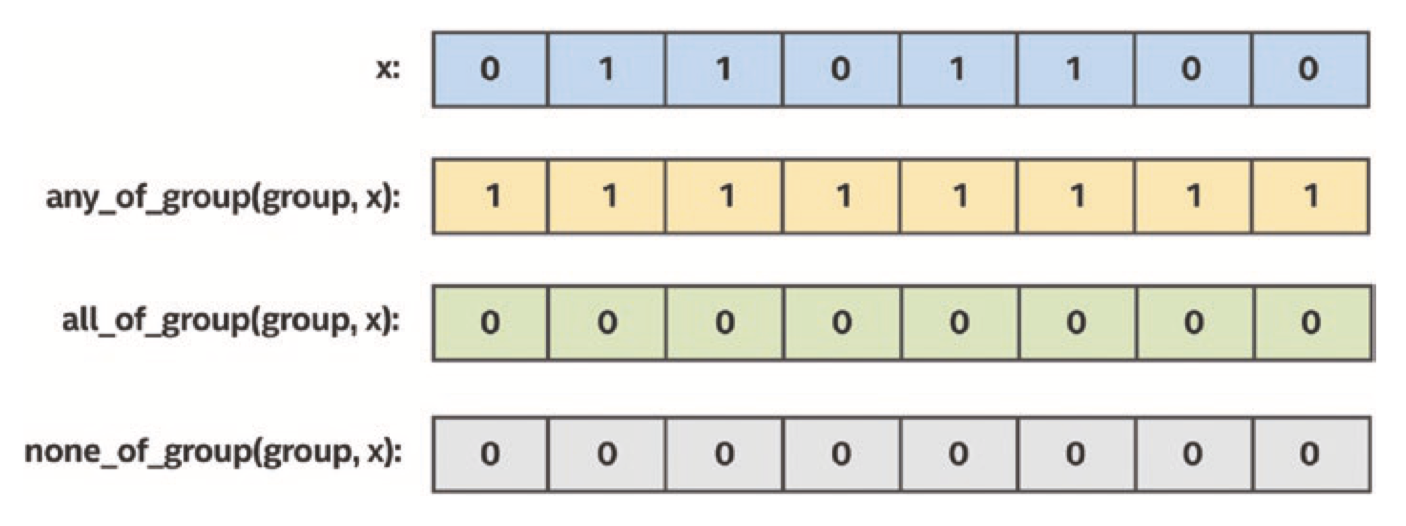
\includegraphics[width=0.9\textwidth]{figs/F9.13.png}
	\caption{\textit{any\_of\_group、all\_of\_group和none\_of\_group功能的比较 }}
\end{figure}

SYCL 2020 还支持这些函数的另一种变体,其中组中的Work-Items协作评估一系列数据,
例如标准 C++ all\_of、any\_of 和 none\_of 算法。 
这些函数被命名为 joint\_any\_of、joint\_all\_of 和 joint\_none\_of,
以区别于组中每个Work-Items保存要直接比较的数据的变体。

例如,投票函数对于某些迭代算法非常有用,可以确定组中所有Work-Items的解决方案何时收敛。 
Work-Groups和Sub-Groups支持投票功能。

\subsubsection{洗牌 Shuffles}
Sub-Groups最有用的功能之一是能够在各个Work-Items之间直接通信,而无需显式内存操作。 
在许多情况下,例如Sub-Groups矩阵乘法Kernel,这些洗牌操作使我们能够从Kernel中删除Work-Groups本地内存使用,
并避免不必要的重复访问全局内存。 这些shuffle 函数有多种类型可供选择。

\begin{figure}[H]
	\centering
	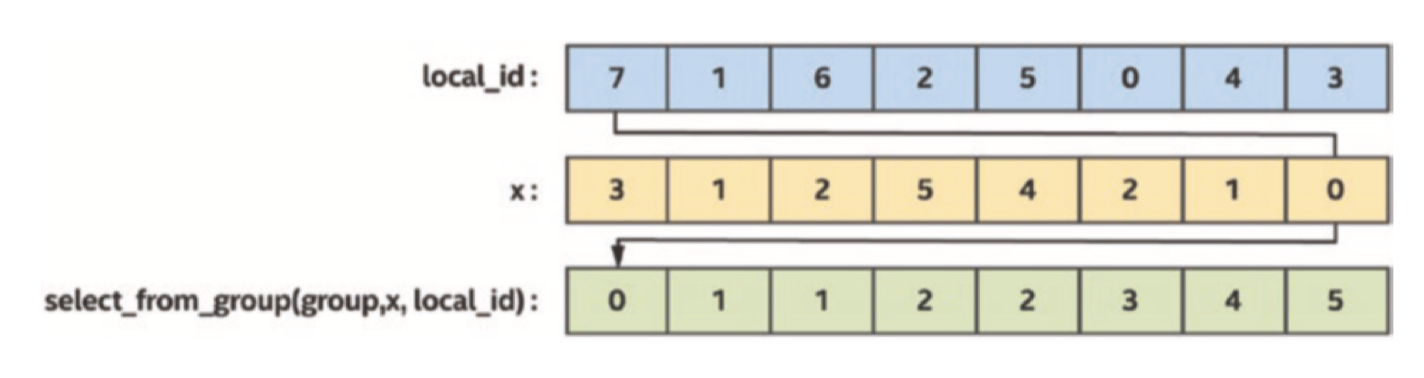
\includegraphics[width=0.9\textwidth]{figs/F9.14.png}
	\caption{\textit{使用泛型select\_from\_group根据预先计算的索引对值进行排序 }}
\end{figure}

最通用的 shuffle 函数称为 select\_from\_group,如图 9-14 所示,
它允许Sub-Groups中任意一对Work-Items之间进行任意通信。 
然而,这种通用性可能会降低性能,我们强烈鼓励尽可能使用更专业的shuffle 函数。

在图 9-14 中,通用洗牌用于使用预先计算的排列索引对Sub-Groups的值进行排序。 
针对Sub-Groups中的一个Work-Items显示了箭头,其中洗牌的结果是 local\_id 等于 7 的Work-Items的 x 值。

请注意,Sub-Groups group\_broadcast 函数可以被视为通用 select\_from\_group 函数的专用版本,
其中Sub-Groups中所有Work-Items的随机索引相同。 
当已知Sub-Groups中所有Work-Items的洗牌索引相同时,使用 group\_broadcast 
而不是 select\_from\_group 可为编译器提供附加信息,并可能提高某些实现的性能。

\begin{figure}[H]
	\centering
	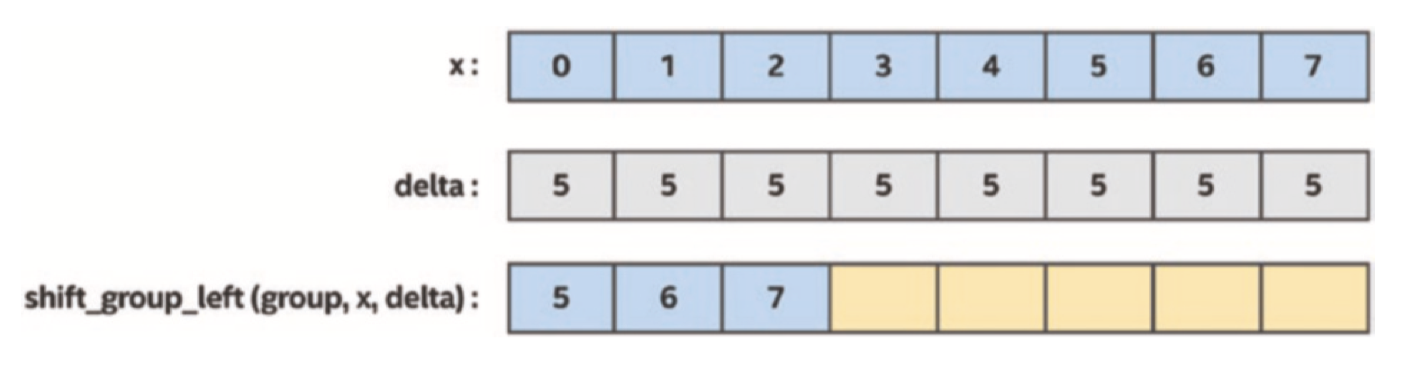
\includegraphics[width=0.9\textwidth]{figs/F9.15.png}
	\caption{\textit{使用 shift\_group\_left 将Sub-Groups的 x 值按 5 个项目移动 }}
\end{figure}

shift\_group\_right 和 shift\_group\_left 函数有效地将Sub-Groups的内容沿给定方向移动固定数量的元素,
如图 9-15 所示。 请注意,返回到Sub-Groups中最后五个Work-Items的值未定义,并在图 9-15 中显示为空白。 
移位对于并行化具有循环携带依赖性的循环或实现常见算法(例如独占或包含扫描)非常有用。

\begin{figure}[H]
	\centering
	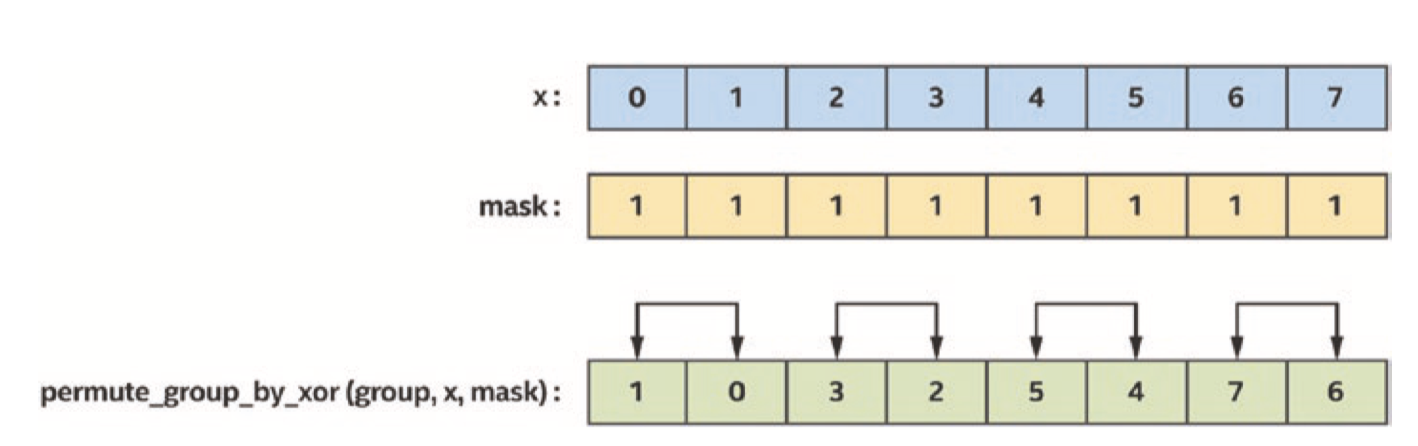
\includegraphics[width=0.9\textwidth]{figs/F9.16.png}
	\caption{\textit{使用permute\_group\_by\_xor交换相邻的 x 对 }}
\end{figure}

\begin{figure}[H]
	\centering
	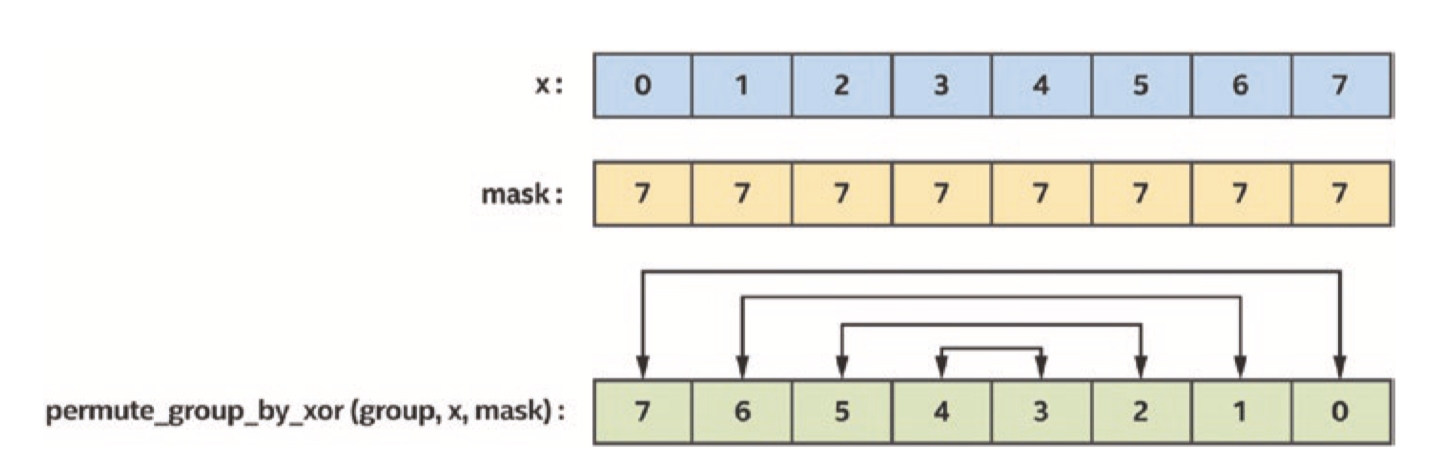
\includegraphics[width=0.9\textwidth]{figs/F9.17.png}
	\caption{\textit{使用permute\_group\_by\_xor反转 x 的值 }}
\end{figure}

permute\_group\_by\_xor 函数交换两个Work-Items的值,
由应用于Work-Items的Sub-Groups本地 ID 和固定常量的 XOR 运算的结果指定。 
如图9-16和图9-17所示,可以使用XOR来表达几种常见的通信模式,例如交换相邻值对或反转Sub-Groups值。

由于shuffle 函数非常专业,因此它们仅适用于Sub-Groups,不适用于Work-Groups。

\begin{remark}[使用广播、投票和集体进行Sub-Groups优化]
应用于Sub-Groups的 Broadcast、Vote 和其他集体函数的行为与应用于Work-Groups时的行为相同,
但它们值得额外关注,因为它们可能会在某些编译器中启用积极的优化。
例如,编译器可能能够减少广播到Sub-Groups中所有Work-Items的变量的寄存器使用量,
或者能够根据 any\_of\_group 和 all\_of\_group 函数的使用情况推断控制流分歧。
\end{remark}

\subsection{总结}
本章讨论了组中的Work-Items如何进行通信和协作以提高某些类型Kernel的性能。

我们首先讨论了 ND 范围Kernel如何支持将Work-Items分组为Work-Groups。 
我们讨论了将Work-Items分组到Work-Groups中如何改变并行执行模型,
从而保证Work-Groups中的Work-Items以支持通信和同步的方式调度执行。

接下来,我们讨论了Work-Groups中的Work-Items如何使用Barrier进行同步以及Barrier如何在Kernel中表达。 
我们还讨论了如何通过Work-Groups本地内存执行Work-Groups中Work-Items之间的通信,
以简化Kernel并提高性能,并且讨论了如何使用本地访问器表示Work-Groups本地内存。

我们讨论了ND范围Kernel中的Work-Groups如何进一步划分为Work-ItemsSub-Groups,
其中Work-ItemsSub-Groups可以支持额外的通信模式或调度保证。

对于Work-Groups和Sub-Groups,我们讨论了如何通过使用集体功能来表达和加速常见的沟通模式。

本章中的概念是理解第 14 章中描述的常见并行模式以及理解如何针对第 15、16 和 17 章中的特定设备进行优化的重要基础。